

\section{Background to the Fusion Concept}

\subsection{Mirrors}
This section presents an overview of key literature in the development of magnetic mirror fusion reactors. This includes their early development, early confinement challenges, how the concept was sidelined in favour of tokamak development, and how there has been a recent return to the concept, with exciting new prospects. 

\begin{itemize}
    \item In "Fusion Research in Open-Ended Systems", 1969, by T.K. Fowler, the focus is on low-beta fusion research in open-ended magnetic geometries, known as magnetic mirrors \cite{fowler1969fusion}. This work provides an overview of magnetic mirror research, discussing methods, achievements, and rationale. It introduces magnetic mirrors for the confinement of hot fusion plasmas in configurations where plasma is held between a pair of coils, creating stronger magnetic fields near the coils. The configuration allows for the escape of certain velocity particles, known as the mirror loss cone, and contrasts with closed systems like toroidal configurations.

 \item In "Concept for a High-Power-Density Mirror Fusion Reactor", 1973, R.F. Post, T.K. Fowler, J. Killeen, and A.A. Mirin propose a new mirror-type fusion reactor design \cite{post1973concept}. Utilizing advancements in neutral-beam technology, this concept improves plasma stability, power density, and the energy gain factor (Q) over previous designs.

 \item "Mirror Reactor Studies", 1976, by R.W. Moir and colleagues at Lawrence Livermore Laboratory introduces a fusion mirror reactor with 150-keV neutral-beam injectors, providing over 1 GW of continuous power \cite{moir1976mirror}. The reactor features a three-stage modularized Venetian blind plasma direct converter with a 59\% efficiency and a novel method for removing the lune-shaped blanket, addressing the challenge of low Q and high recirculating power.

 \item In "Improved Tandem Mirror Fusion Reactor", 1979, D.E. Baldwin and B.G. Logan discuss barrier potentials in tandem mirror reactors to reduce ion energy and density requirements \cite{baldwin1979improved}. This innovation, involving raising the plug-electron temperature, marks a significant advancement in magnetic mirror fusion technology.

 \item In "Magnetic Mirror Fusion - Status and Prospects", 1980, Post compares the concept of magnetic mirror fusion to closed magnetic systems like tokamaks \cite{post1980magnetic}. It is explained that mirror confinement, an open system, features magnetic field lines extending beyond the confinement area, contrasting with closed systems where these lines are contained. The importance of the magnetic mirror effect for longitudinal confinement is highlighted, with emphasis on the necessity for particles to have sufficient rotational energy for effective trapping. The "loss cone" in velocity space, influenced by the mirror ratio and particle energy ratio, is also described. The paper notes that the imbalance in electron and ion loss rates is compensated by the development of a positive ambipolar potential, affecting the overall plasma loss rate. It is concluded that higher temperatures, which reduce ion-ion collision rates and boost fusion rates, could improve the fusion power balance in mirror confinement systems.

 \item "Experimental Progress in Magnetic-Mirror Fusion Research", 1981, by Thomas C. Simonen emphasizes the progression from basic mirror cells to advanced designs in magnetic mirror systems like tandem mirrors \cite{simonen1981experimental}. It discusses improvements in plasma containment and the reduction of end losses, along with the technical aspects of magnetic mirror confinement.

 \item "The Engineering of Magnetic Fusion Reactors", 1983, by Robert W. Conn delves into the construction of magnetic fusion reactors using the tandem mirror method, highlighting challenges and techniques in maintaining plasma temperature and energy capture \cite{conn1983engineering}.


 \item "Mirror-Based Fusion: Some Possible New Directions", 1999, by Richard F. Post highlights innovative approaches in magnetic mirror fusion - offering several benefits, including suppression of interchange-type MHD instability modes due to positive field-line curvature, and the ability to introduce and control particle beams for improved fueling and ash removal \cite{post1999mirror}. Additionally, Post suggests a shift towards low-Q open-ended systems for their relaxed confinement requirements and better-understood physics. This approach brings potential for more efficient, smaller, and less expensive fusion systems and opens possibilities for using alternative fusion fuels.
 
 \item In "Fifty Years of Magnetic Fusion Research (1958-2008): Brief Historical Overview and Discussion of Future Trends", 2010, by Laila A. El-Guebaly, magnetic mirror fusion is discussed as one of the original magnetic confinement concepts alongside tokamak, stellarator, and pinch \cite{el2010fifty}. Tandem Mirror (TM) research, a variation of magnetic mirror fusion, began in the 1950s. By the mid-1970s, the TM concept was proposed, offering advantages like high beta (30–70\%), no driven plasma current, and the potential for direct conversion of charged particle power into electricity. The TM design consists of a long central cell with solenoidal coils terminated by end mirror cells and direct conversion systems. In the 1980s, major TM experimental facilities were built in the US, including MFTF-B and TMX-U, and conceptual power plant designs like WITAMIR, MARS, MINIMARS, and Ra were developed. However, by the late 1980s, the US Department of Energy shifted focus away from TMs to concepts with seemingly fewer challenges, like tokamaks. Despite the early promise, the TM concept has seen limited growth in recent years, with existing magnetic traps like the gas-dynamic trap and multi-plug trap at the Budker Institute of Nuclear Physics not being TMs.

 \item "Modern magnetic mirrors and their fusion prospects", 2010, by A.V. Burdakov et al. present advancements in magnetic mirror technology, focusing on the Gas Dynamic Trap (GDT) and the Multi-Mirror Trap from the Budker Institute of Nuclear Physics \cite{burdakov2010modern}. These developments represent key steps in making magnetic mirror technology viable for practical fusion applications.

  

  \item In "Concept of Fusion Reactor Based on Multiple-Mirror Trap", 2011, A.V. Burdakov and colleagues focus on advancements in multiple-mirror confinement for fusion reactors, using the GOL-3 device in Novosibirsk as a case study \cite{burdakov2011concept}. It reports significant improvements in plasma behavior, facilitated by new collective phenomena and enhanced plasma heating methods. These advancements, including effective heat transport control and magnetohydrodynamic stabilization, have improved the viability of multiple-mirror confinement systems for practical fusion reactor applications. The study also provides a perspective on the development of large-scale fusion devices using this technology.

 \item In "Gas-dynamic Trap: An Overview of the Concept and Experimental Results", 2013, A.A. Ivanov and V.V. Prikhodko explore the Gas Dynamic Trap (GDT) - a type of magnetic mirror reactor \cite{ivanov2013gas}. This reactor is characterized by its long distance between mirrors and high mirror ratio, enabling effective plasma confinement. The GDT's design facilitates plasma stability and offers promising applications in neutron source development for fusion materials and hybrid fusion-fission systems. The paper also reviews experimental results from GDT trials, providing insights into its potential in future fusion research.

  \item In "Progress in Mirror-Based Fusion Neutron Source Development", 2015, by the Budker Institute of Nuclear Physics  advancements in developing a 14 MeV neutron source for fusion material studies are detailed \cite{anikeev2015progress}. This source, based on the Gas Dynamic Trap (GDT), a specialized magnetic mirror system, has achieved stable confinement of hot-ion plasmas with relative pressures exceeding 0.5 and elevated the electron temperature to 0.9 keV. These achievements, including the highest electron temperature reached in axisymmetric open mirror traps, position the GDT-based neutron source as a promising tool for material testing and fusion-fission hybrid systems.

 \item In "Magnetic-confinement Fusion", 2016, by J. Ongena et al., the concept and history of magnetic mirrors in fusion research is presented \cite{ongena2016magnetic}.  The paper describes magnetic mirrors as working by increasing the magnetic field strength at both ends of a confinement region, using additional coils to create a 'magnetic bottle'. This design repels plasma particles with an identical pole to the strong end magnetic fields, trapping them within the bottle. Despite this innovative approach, achieving effective confinement in mirror machines proved challenging, primarily due to instabilities caused by end losses. Particles with velocities mainly along the magnetic field line would not be stopped by the end mirrors and escape, leading to a non-Maxwellian velocity distribution and instabilities. This issue ultimately led to the abandonment of the magnetic-mirror approach in 1986 when the U.S. decided not to operate the Mirror Fusion Test Facility B (MFTF-B).

 \item In "Encouraging Results and New Ideas for Fusion in Linear Traps", 2018, by P.A. Bagryansky and colleagues reviews recent advancements in linear trap technologies \cite{bagryansky2019encouraging}. This study highlights the efficiency of multiple-mirror confinement with gas-dynamic traps and introduces the helical-mirror variant for improved confinement of rotating plasmas, laying a foundation for future fusion energy exploration and development.


 \item In "Fusion by beam ions in a low collisionality, high mirror ratio magnetic mirror", 2022, Egedal et al.'s study introduces the Fast Beam Ion Solver (FBIS) model to improve the understanding of ion behavior in magnetic mirror geometries, contributing to the design of WHAM++, a cost-effective magnetic mirror device \cite{egedal2022fusion}.

\end{itemize}
\label{MIF_lit_review}

\subsection{MIF Review}

\subsection{Introduction to MIF with LINUS Compression Scheme}

The approach to MIF with magnetic mirrors presented here is based on the literature presented in section \ref{MIF_lit_review}, and the Stabilized Liner Compressor, technology that first was developed into engineering prototypes at the Naval Research Laboratory in the late 1970s and 1980s.  There are three major aspects to the technology: the magnetic mirror coils, the compressor, and the plasma configuration undergoing a compression. The latter two are discussed in this section.\\


The concept was first described by Boris and Shanny in 1972 \cite{Boris1972} \cite{Boris1972a} then in 1973 by Boris \cite{Boris1973} and Robson \cite{Robson1973}.  The stability of the rotating liner was presented in 1974 by Barcilon \cite{Barcilon1974} and by Book and Winsor \cite{Book1974}.  The imploding liner experiment SUZY II was described in 1975 by Ford \cite{Ford1974} and Young and Ford \cite{Young1974}. In 1975 Barcilon presented results of two-dimensional simulations of liners imploding onto a cusp plasma with relevance to controlled fusion \cite{Barcilon1975}, and the same year, Turchi presented a mathematical model of the compression of a theta-pinch with splayed ends and implications made for fusion reactors \cite{Turchi1975}.  In 1976, Robson and Turchi \cite{Robson1976} outlined the LINUS approach to a fusion reactor concept and outlined the advantages: no first first wall problem because the first wall is continuously replenished; activation of the stationary part of the machinery is minimized due to protection by the thick liquid metal liner; very high compression ratios can be obtained with great efficiency relative to compression systems with stationary coils; and, reversible compression-expansion cycles lead to very "compact fusion systems". In 1976, Schaffer published the equilibrium calculations of a cold-ended dense liner fusion plasma, considering alpha-particle slowing by the plasma \cite{Schaffer1976}.  The same year, he published on self-driving liner compression systems \cite{Schaffer1976a} in which liquid liners for compression of magnetic flux and plasma can contrain sufficient energy to compress both the liner and the plasma when stability to Raleigh-Taylor is achieved. In 1976, Turchi reported on stabilization of the liner with electrogmetic implosion of sodium-potasiium liners, and high pressure gas-driven water liners \cite{Turchi1976}; and, Turchi and Robson summarized successful demonstration of implosion of solid metal liners with radial compression ratios of 28 and fields in excess of 1.3Mgauss (130T) \cite{Turchi1976a}, although concluded that implosion of solid liners would not be relevant to fusion energy systems.  \\

In 1977, Book reported on stabilized imploding liner fusion systems based on the liquid metal liner, that "could lead to a very compact thermonuclear reactor operating in the manner of a reciprocating engine." \cite{Book1977}. The same year: Burton reported on implosion results with water and an annular piston: radial implosion of the free inside surface of the liquid was achieved by axial displacement of an annular piston, driven by helium \cite{Burton1978};  Ford reported on high explosive pulsed gas generator for the LINUS-0 rotationally-stablized liner magnetic flux compression experiment, which produced repeatable piston accerations from rest with no damage to the hardware \cite{Ford1977};  Parish and Davidson performed neutronic evaluation for the transmutation of fission products \cite{Parish1977}; Robson published on the a fusion reactor based on the LINUS principle \cite{Robson1977}; and, Turchi presented the engineering design of the LINUS-0 prototype liner implosion system \cite{Turchi1977} as well as performing a technological review of stabilized imploding liner systems, involving the periodic adiabatic compression of high beta plasma, and summarized tritium breeding, and neutron shielding \cite{Turchi1977a}.  \\

In 1978, Book reported on theoretical studies of a field reversed configuration as a plasma target \cite{Book1978}; Book and Turchi published on a field-free plasma separated from the liner by a thin plasma-free region of high magnetic field, describing the design of the imploding liner \cite{Book1978a}; Burton and Turchi presented the design for a 700MWe fusion reactor with a pulse rate of 1Hz \cite{Burton1978}; Cooper and Book presented calculations of the Joule heating resulting from magnetic flux diffusion into an imploding liquid liner \cite{Cooper1978}; and, Schaffer presented 1D calculations of the compression of a plasma column by a rotating liquid metal liner showing that fusion power production is possible with reasonable net efficiencies \cite{Schaffer1978}.\\


In 1979, Book and Bernstein published on perturbations about a time-varying state of a compressible medium, finding that results  reduce to the Rayleigh-Taylor instability \cite{Book1979}; Book presented results from the LASL Fast Liner and LINUS slow liner experiments \cite{Book1979a}; Book and Turchi published analytic and numerical results on the dynamics of rotationally stabilized implosions of compressible cylindrical liquid shells \cite{Book1979b}, reporting that near turnaround, the inner portion of the liner becomes significantly compressed, altering the implosion dynamics, creating a pressure pulse that propagates outwards, like a 'water hammer'; Davidson and Parish again report on the requirements and performance of a transmutation waste management system \cite{Davidson1979};  Sethian and Robson continue the discussion of the use of electron beams to create magnetically confined plasmas inside imploding liners \cite{Sethian1979}; Turchi published on the 'Optimization of stabilized imploding liner fusion reactors' \cite{Turchi1979}, discussing the trade-offs between reactor size and initial plasma temperatures, and implosion radius-ratio and liner compressibility;  and, Turchi published on results from the NRL LINUS research effort, indicating theoretical plasma behavior during liner compression.\\

In 1980, Brennan presented engineering analyses for imploding systems, that included material considerations, injection systems, rotor geometries and mechanical stresses \cite{Brennan1980}; Cooper presented on theoretical studies of the LINUS liner dynamics \cite{Cooper1980}; Hasasaki and Book considered transport modeling in a field reversed configuration undergoing a compression, finding that a high field, low-density buffer region near the wall can be used as a heat insulator \cite{Hamasaki1980}; Itoh published on a blade system for directing flows in the radial direction for imploding liquid metal systems obviating the high speed rotary mechanisms \cite{Itoh1980a} and also on the effects of an oscillating azimuthal magnetic field \cite{Itoh1980b}, which was co-authored by Turchi; Robson and Turchi presented a conceptual design for an imploding fusion reactor, using liquid lithium, for which the liner acts as the confining magnet, thr tritium breeding blanket and the heat transfer medium, as well as a continuously replaced first wall \cite{Robson1980}; Turchi presented a review of the NRL liner implosion program, reporting on LINUS-0 and HELIUS with initial bores of 30cm and 15cm respectively; Miller and Krakowski performed a reactor cost analysis of the LINUS concept based on design points discussed above by Robson and Turchi \cite{Miller1980}, which interestingly provided a LCOE estimate of 59mills/kWh.\\

In 1981, Krakowski followed up with a longer publication on the systems studies for several competing fusion energy concepts that included the LINUS concept \cite{Krakowski1981}; and, Quimby published on a power balance for a full compression cycle, supported by numerical (1D) calculations, that implied a minimum system size \cite{Quimby1981}.\\

In 1983, Itoh published again on imploding liners with blade lattices inclined to the radial direction with application to fusion \cite{Itoh1983}; Robson presented the concept of using rotating relativistic electron beams to create a magnetically-confined plasma inside an imploding liner \cite{Robson1983}; Turchi presened the development of imploding liner systems \cite{Turchi1983}, but by this time, the LINUS program was ramping down, not for any good reason other than the compressor technology was awaiting a suitable plasma target for compression.  Patents were filed on the axisymmetric implosion system by Turchi in 1979 \cite{Turchipat1}, and also for use in a propulsion system in 2008 \cite{Turchipat2}.\\

In 2008, Turchi presented on the 'issues of liner-plasma compression' \cite{Turchi2008}, which captured among many matters, the development of an equilibrium layer of vapor adjacent to the liner surface at high magnetic fields; Turchi published separately on the requirements for the plasma \cite{Turchi2008a} based on the plasma flow switch;  Turchi revisited the plasma flow switch again in 2010 \cite{Turchi2010}.\\

In 2016, the ARPA-E ALPHA program started up, which included a revisit of the LINUS concept.  Turchi presented on a controlled fusion reactor based on the stabilized liner compression of a magnetized plasma \cite{Turchi2016a}, and later published analytic and simulation results from the program in 2017 \cite{Turchi2017}.  Finally, the engineering design of the compressor that was designed with ARPA-E support was published by Kittu \cite{Kiuttu2018}.\\

Much progress has been made in the last 40 years on the plasma target, which mostly has been captured by Steinhauer \cite{Steinhauer2011} \cite{Steinhauer2018}, Asai \cite{Asai2019} and Lau \cite{Lau2019} and Gota \cite{Gota2019}.  Essentially, the collisional-merging formation of FRCs is now well understood, with a range of formation methods, and understanding of the stability (to n=1, n=2 modes) and confinement properties (approaching classical in the closed flux).  Worth mentioning that Woodruff has published on the topic of colliding FRCs, arguably with the first computational simulations of collision, merging and compression \cite{Woodruff2007a} \cite{Woodruff2008/06/b}.



\begin{figure}[h!] 
\begin{center} 
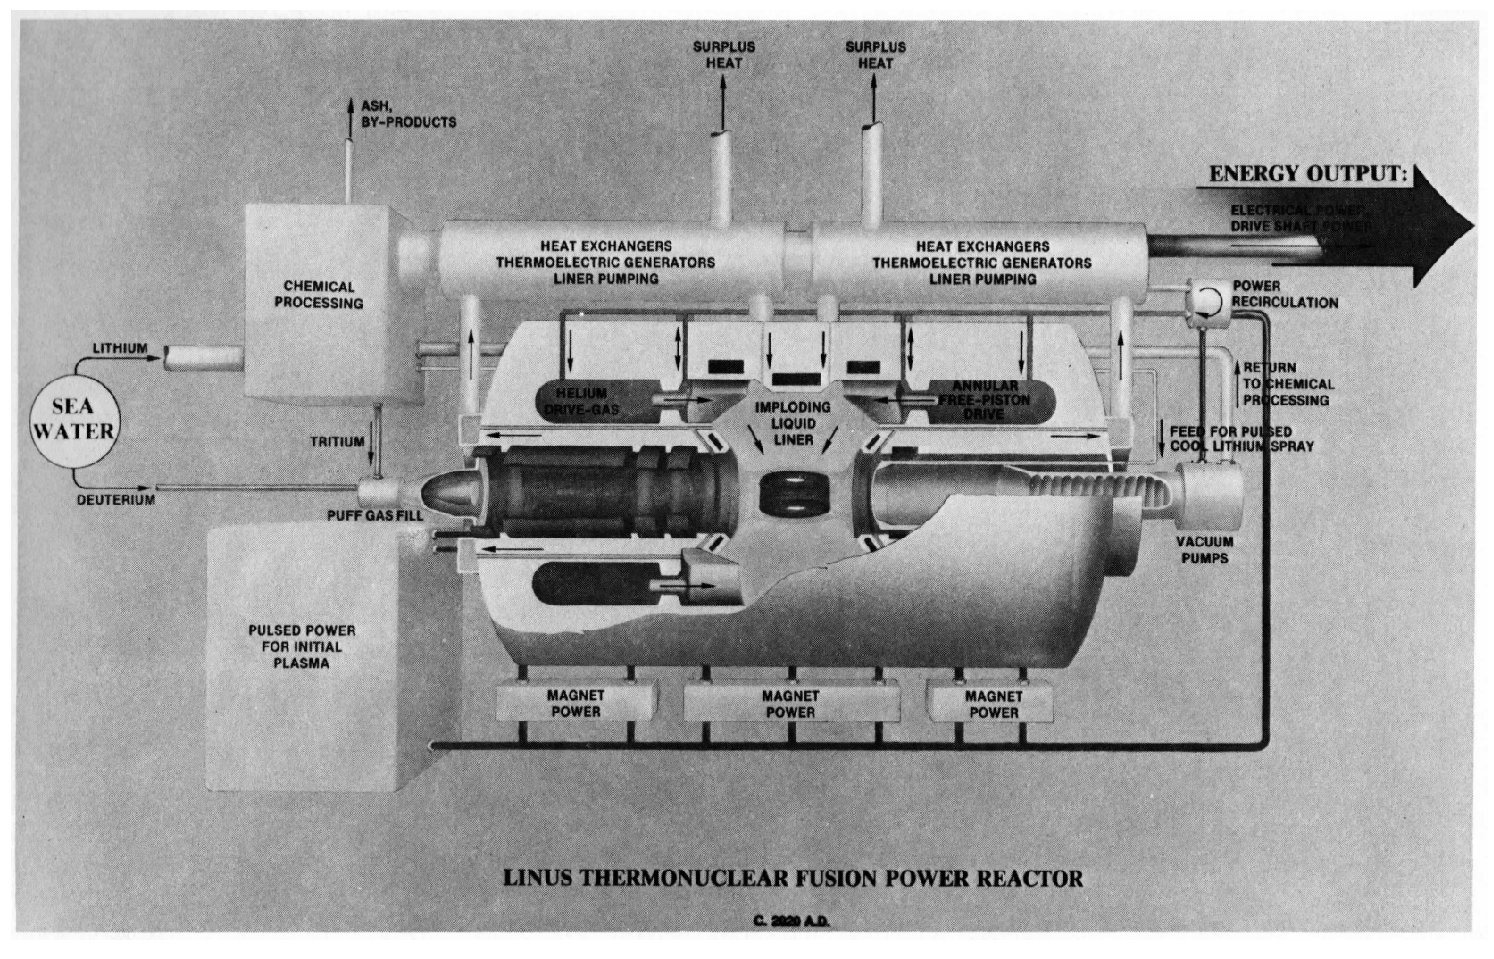
\includegraphics[scale=0.5]{SubreportFigures//LINUS_reactor.pdf} 
\end{center} 
\caption{Reactor embodiment of the Stabilized Liner Compressor based on the LINUS concept.} 
\label{fig::INUS} 
\end{figure} 